%!TEX root = pag0.tex

\chapter{Introduzione}
\label{chapter1}
%In questo report verrà presentato il progetto del corso di Guida e Navigazione. 
Nella vita quotidiana ci troviamo spesso a dover premere dei pulsanti, i.e quelli del citofono, i pulsanti dell'ascensore etc. Le pulsantiere, si pensi a quelle degli ascensori, sono poste in modo da essere premute senza dover alzare il braccio più in alto della linea degli occhi. Se pensiamo ai bambini, per premere un pulsante si mettono sulle punte dei piedi. Cosa succede se una persona con una carrozzina non arriva a premere un pulsante?. Questo progetto si occupa di aiutare i diversamenti abili ad essere più indipendenti. Lo scopo del progetto è l'identificazione della posizione del pulsante desiderato e l'invio di tali informazioni al controllore del braccio robotico. L'utente con il supporto di un tablet, preme su di esso il bottone desiderato. Una volta identificato il pulsante premuto, la camera fornisce al robot le informazioni di posizione ad orientazione in modo da posizionarsi sul percorso corretto. La camera utilizzata è monoculare pertanto non si hanno informazioni sulla distanza. Per ovviare a questa mancanza si è deciso di utilizzare un algoritmo esterno chiamato \emph{PTAM} ~\cite{PTAM} capace di utilizzare le informazioni delle features trovate per stimare una posizione relativa.
Il codice si divide in tre fasi:
\begin{itemize}
\item Fase di plan
\item Fase di tracking
\item Interfacciamento con l'algoritmo esterno
\item Fase di triangolazione e scalatura
\end{itemize}
Nella prima fase si utilizzano algoritmi di elaborazione dell’immagine, in modo da ottenere la posizione
dell’oggetto in coordinate camera. Nella seconda fase si ricercano nella seconda immagine le features di interesse e si stima la posizione del bottone tramite algoritmi di matching. Nella terza fase si elaborano i dati ricevuti dall'algoritmo esterno, Ptam. Nella quarta e ultima fase i dati elaborati vengono triangolati e, opportunamente scalati per trovare la posa relativa.

I sistemi di acquisizione maggiormente impiegati possono essere suddivisi in due categorie. Una prima categoria fa riferimento al modo in cui viene usato il sistema di visione. Se la telecamera inquadra direttamente l’oggetto dal punto di vista del manipolatore, si parla di sistemi \lq \lq eye-in-hand \lq \lq. In questo caso la posizione
e l’orientamento della telecamera sono solidali con l’end-effector del manipolatore.
Un’altro tipo di configurazione consente di avere la telecamera che mantiene una posizione fissa nell’ambiente e al più con orientamento variabile, ed inquadra sia il manipolatore che l’oggetto target. Quest’ultima modalità
viene denominata \lq \lq eye-to-hand \lq \lq.. È possible notare le differenze nelle capacità visive del manipolatore in questa due modalità di configurazione dalla figura ~\ref{fig:eye_in_hand}
\begin{figure}[H]
   \centering
   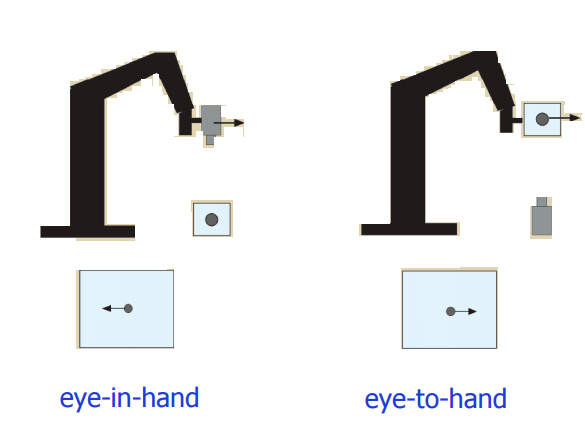
\includegraphics[width=.7\columnwidth]{eyetoinhand.png}
   \caption{Differenza tra le due categorie di posizionamento della camera}
   \label{fig:eye_in_hand} 
\end{figure}
Nelle tecniche tradizionali di asservimento visivo viene invece spesso effettuata la misura diretta della posizione del manipolatore fornita dalla telecamera, per migliorare l’accuratezza del posizionamento del end-effector. I dati forniti dalla telecamera, in questo caso, incrementano la precisione delle informazioni fornite dall’apparato meccanico del robot, in quanto non risultano affetti dai tipici errori dovuti ad un’imprecisa conoscenza dei parametri fisici del manipolatore, che risultano particolarmente evidenti nel caso in cui si debba considerare anche la flessibilità della struttura.
L’ambiente, in cui si muove il robot, possiede alcune caratteristiche che inevitabilmente influenzano il processo di comprensione della scena. Nei sistemi robotici dotati di sensori di visione vengono spesso applicate le seguenti ipotesi:
\begin{itemize}
\item il robot deve essere un agente autonomo, per cui non è possibile alcun intervento esterno per controllarlo;
\item gli oggetti da riconoscere presenti nell’immagine devono essere fortemente caratterizzati;
\item le condizioni di illuminazione della scena sono in genere fortemente variabili, questo influisce molto sul riconoscimento degli oggetti;
\item le occlusioni, rendono impossibile il riconoscimento degli oggetti basandosi sull’analisi della loro forma
\end{itemize}
In questo progetto è stato impiegato una configurazione del primo tipo. 





% \newpage 



\subsection{Organizzazione del report}
Nel capitolo ~\ref{chapter2} si spiega il modello della camera utilizzata e le sue caratteristiche.  Nel capitolo ~\ref{chapter3} verrà spiegato il meccanismo di tracking e del matching mentre nel capitolo ~\ref{chapter4} viene introdotto l'algoritmo sviluppato. Nel capitolo ~\ref{chapter5} vengono esposti gli esperimenti e nel ~\ref{chapter6} le conclusioni. In appendice A vi è una panoramica del codice sviluppato.